\begin{frame}{Ordre logique}
  Quel est l'ordre logique pour les activités suivantes?
  \begin{columns}
    \column{0.5\textwidth}
      {\scriptsize
      \begin{enumerate}
        \item se laver; s'habiller
        \item<2->[$\to$] On se lave, et après on s'habille.
        \item<3-> se coiffer; se laver les cheveux
        \item<4->[$\to$] On se lave les cheveux, et après on se coiffe.
        \item<5-> se lever; se réveiller
        \item<6->[$\to$] On se réveille, et après on se lève.
        \item<7-> se coucher; s'endormir
        \item<8->[$\to$] On se couche, et après on s'endort.
        \item<9-> s'essuyer; se laver
        \item<10->[$\to$] On se lave, et après on s'essuie.
      \end{enumerate}
      }
    \column{0.5\textwidth}
      \begin{minipage}[c][0.6\textheight]{\linewidth}
        \begin{center}
          \only<2>{
            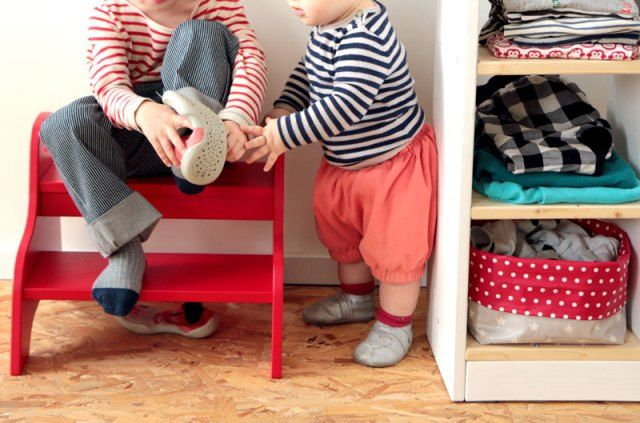
\includegraphics[scale=0.25]{shabiller.jpg}
          }
          \only<4>{
            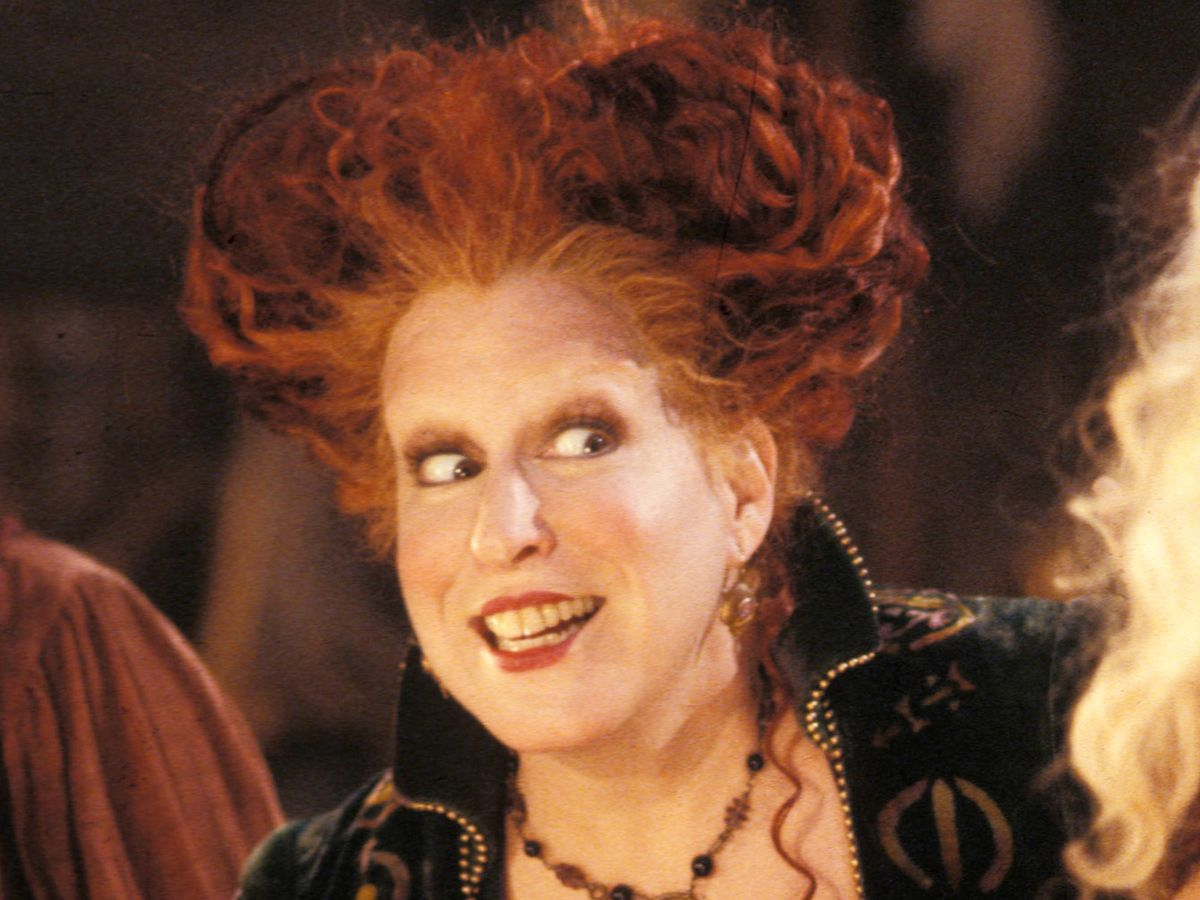
\includegraphics[scale=0.13]{se_coiffer.jpg} \\
            Hocus Pocus
          }
          \only<6>{
            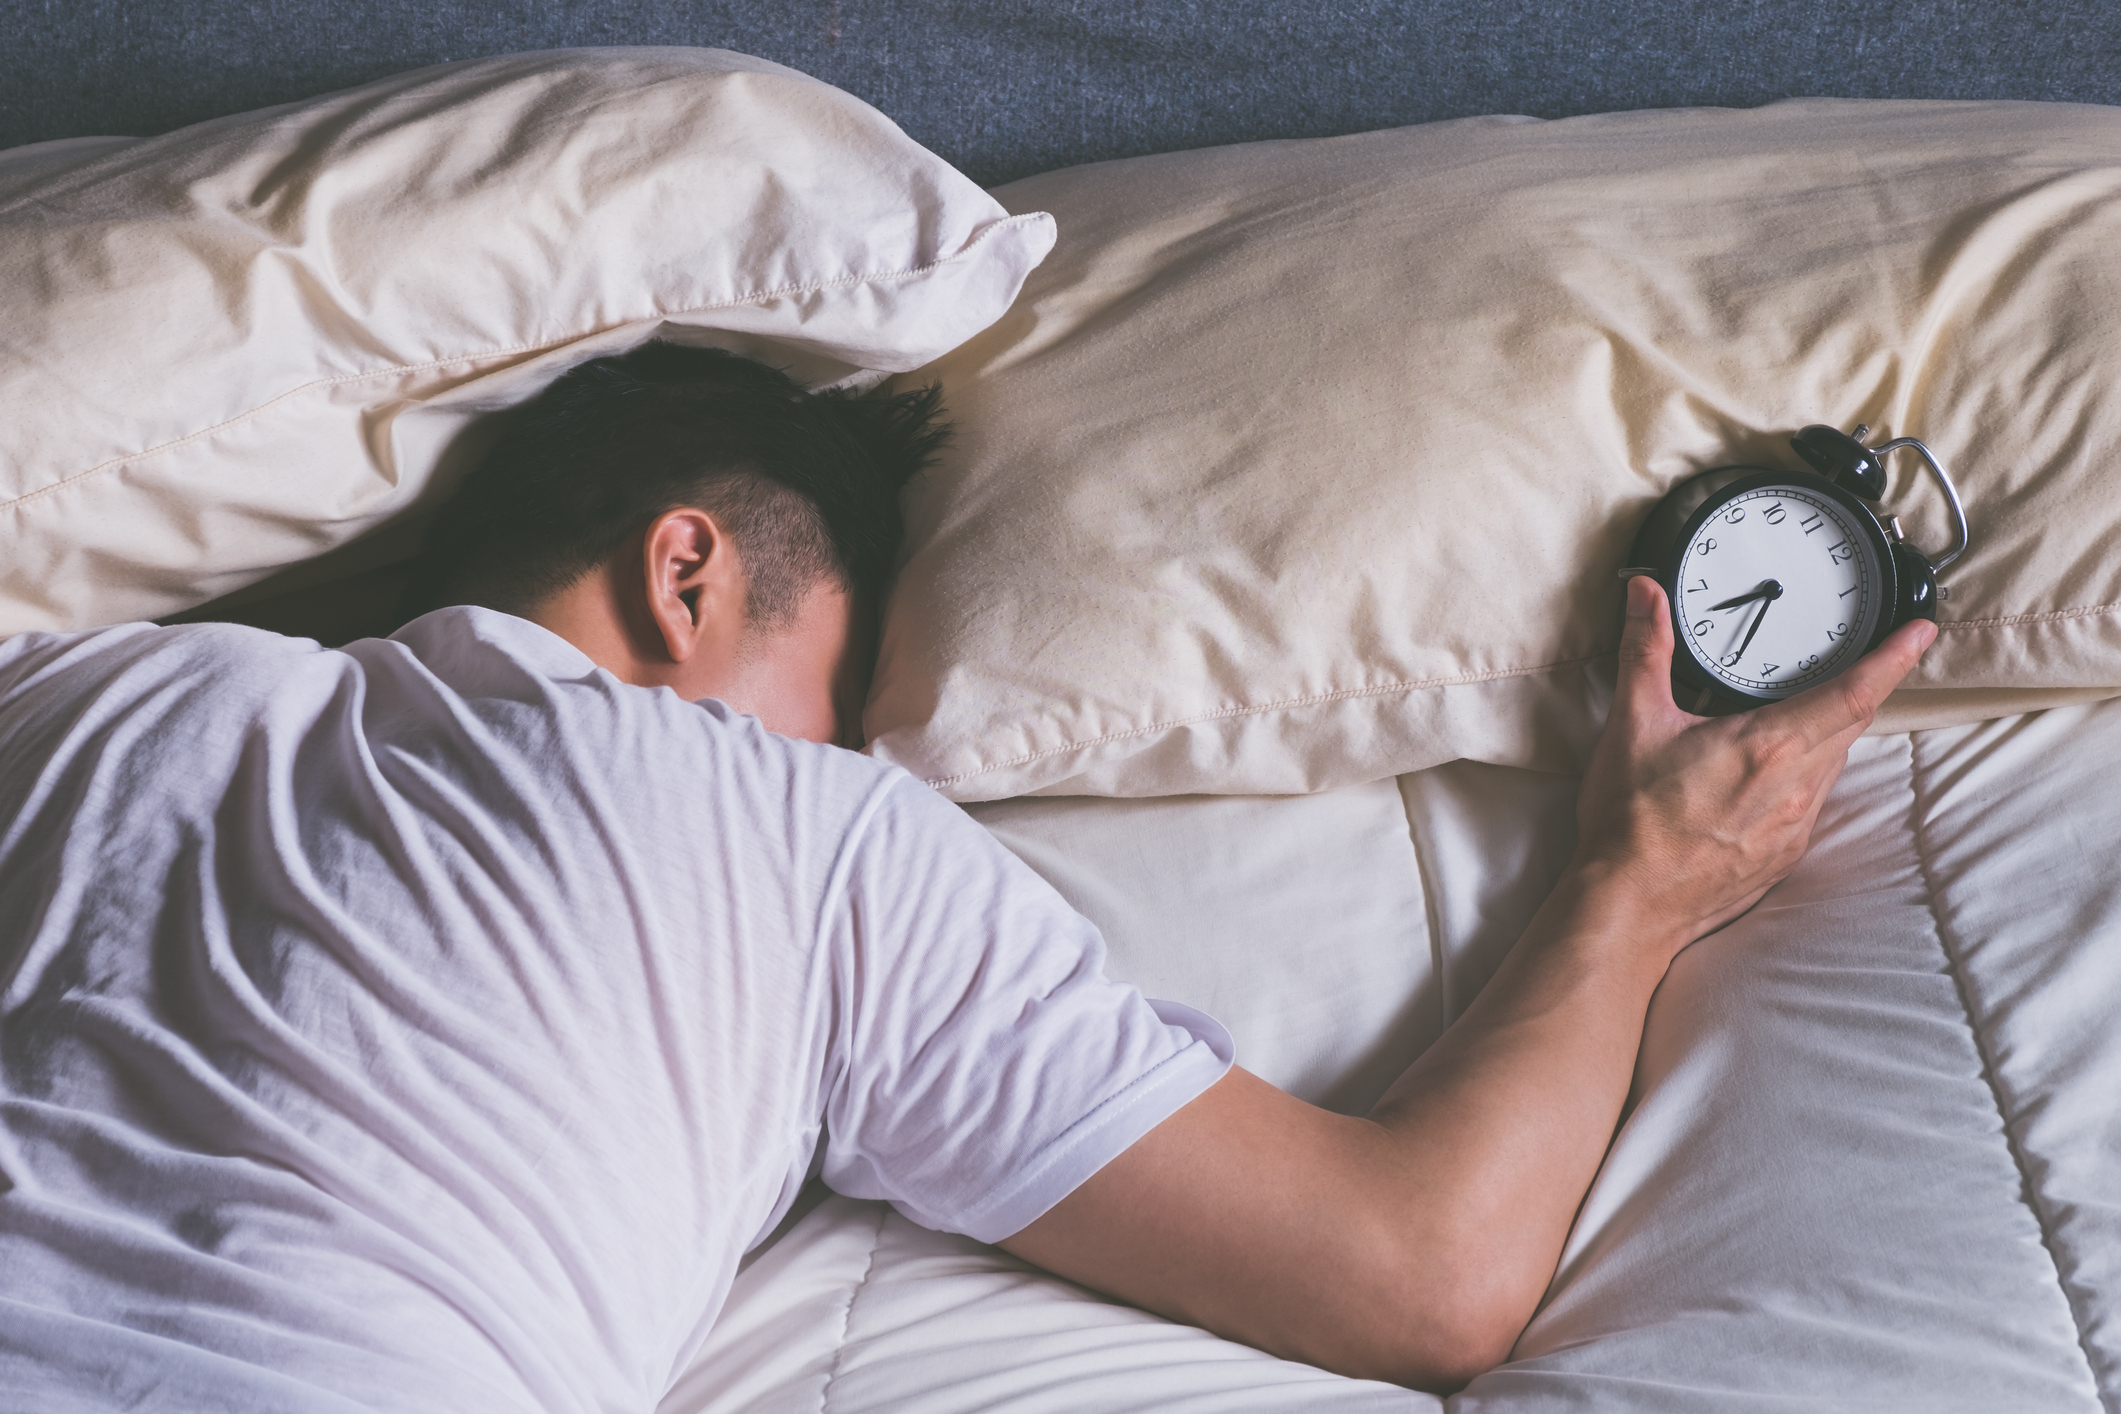
\includegraphics[scale=0.3]{se_reveiller.jpg}
          }
          \only<8>{
            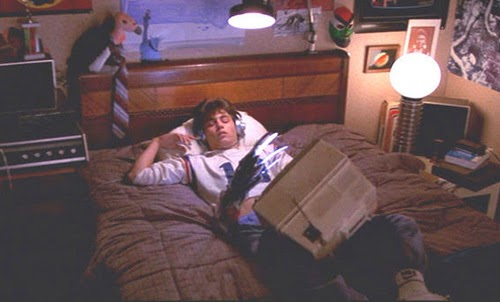
\includegraphics[scale=0.35]{freddy_lit.jpg} \\
            A Nightmare on Elm Street
          }
          \only<10>{
            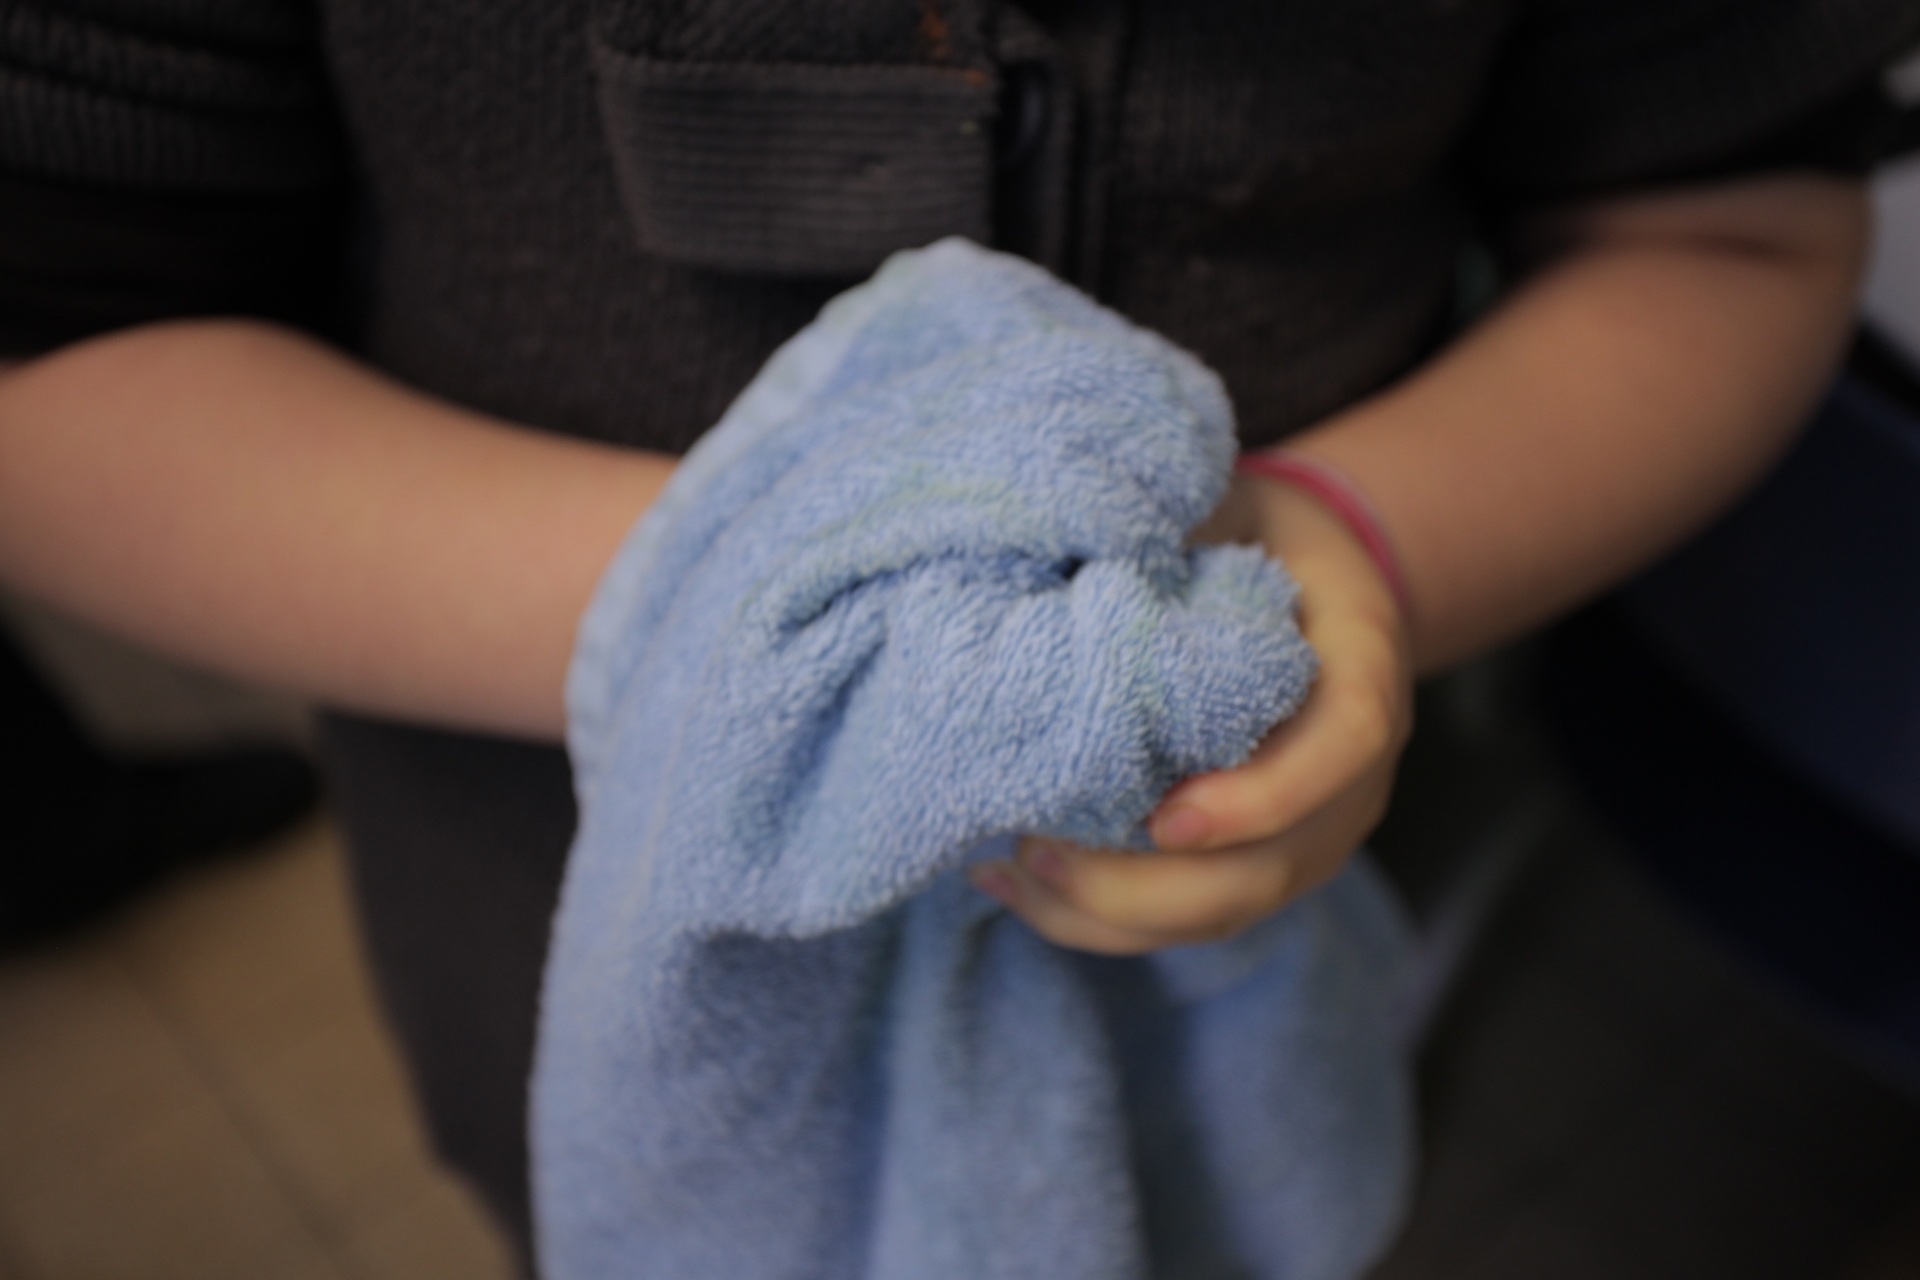
\includegraphics[scale=0.08]{sessuyer.jpg}
          }
        \end{center}
      \end{minipage}
  \end{columns}
\end{frame}